% !TeX spellcheck = <none>
\documentclass[a4paper, 12pt]{article}

%\usepackage{cmap}
\usepackage[T2A]{fontenc}
\usepackage[utf8]{inputenc}
\usepackage[english, russian]{babel}
\usepackage{graphicx}
\usepackage[top=1in, bottom=1in, left=3.2cm, right=2.6cm]{geometry}
\graphicspath{./}
\usepackage{biblatex}
\addbibresource{lib.bib}
\linespread{1.5}
\usepackage{ragged2e}
\justifying
\usepackage{listings}
\usepackage{color}
\usepackage{amsmath}


\begin{document}
	
\begin{titlepage}
	\fontsize{12pt}{12pt}\selectfont
	\begin{figure}[t!]
		\centering
		
\includegraphics[scale=0.8]{bmstu}
	\end{figure}
	
	\noindent\rule{15cm}{3pt}
	\newline\newline
	\noindent 
	ФАКУЛЬТЕТ 
	\underline{«Информатика и системы управления»} \newline
	
	\noindent КАФЕДРА \underline{«Программное обеспечение ЭВМ и информационные технологии»}\newline\newline\newline\newline\newline
	
	\centering {\Large \textbf{Отчет по лабораторной работе № 7}}
	\vspace{4mm}
	
	\centering {\Large \textbf{По курсу:} Моделирование
		\vspace{8mm}}
	\\ \centering {\Large \textbf{На тему:} Моделирование работы информационного центра при помощи GPSS}
	\vspace{20mm}
	
	
	\begin{flushright}
		{\small	\textbf{Студент:}\\ Турсунов Жасурбек Рустамович \\ \textbf{Группа:} ИУ7-76Б
			\vspace{3mm}
			\\\textbf{Преподователь:} \\ Рудаков Игорь Владимирович }
	\end{flushright}
	
	\begin{center}
		\vfill
		Москва, \the\year
		~г.
	\end{center}
\end{titlepage}

\tableofcontents
\clearpage
\newpage


\section{{Задание}}

\hspace*{5mm} В информационный центр приходят клиенты через интервал времени 10 $\pm$ 2 минуты. Если все три имеющихся оператора заняты, клиенту отказывают в обслуживании. Операторы имеют разную производительность и могут обеспечивать обслуживание среднего запроса пользователя за 20 $\pm$ 5; 40 $\pm$ 10; 40 $\pm$ 20. Клиенты стремятся занять свободного оператора с максимальной производительностью. Полученные запросы сдаются в накопитель. Откуда выбираются на обработку. На первый компьютер запросы от 1 и 2-ого операторов, на второй – запросы от 3-его. Время обработки запросов первым и 2-м компьютером равны соответственно 15 и 30 мин. Промоделировать процесс обработки 300 запросов.
\hspace*{5mm} Для выполнения поставленного задания необходимо создать концептуальную модель в терминах СМО, определить эндогенные и экзогенные переменные и уравнения модели. За единицу системного времени выбрать 0,01 минуты.
\begin{figure}[h!]
	\centering 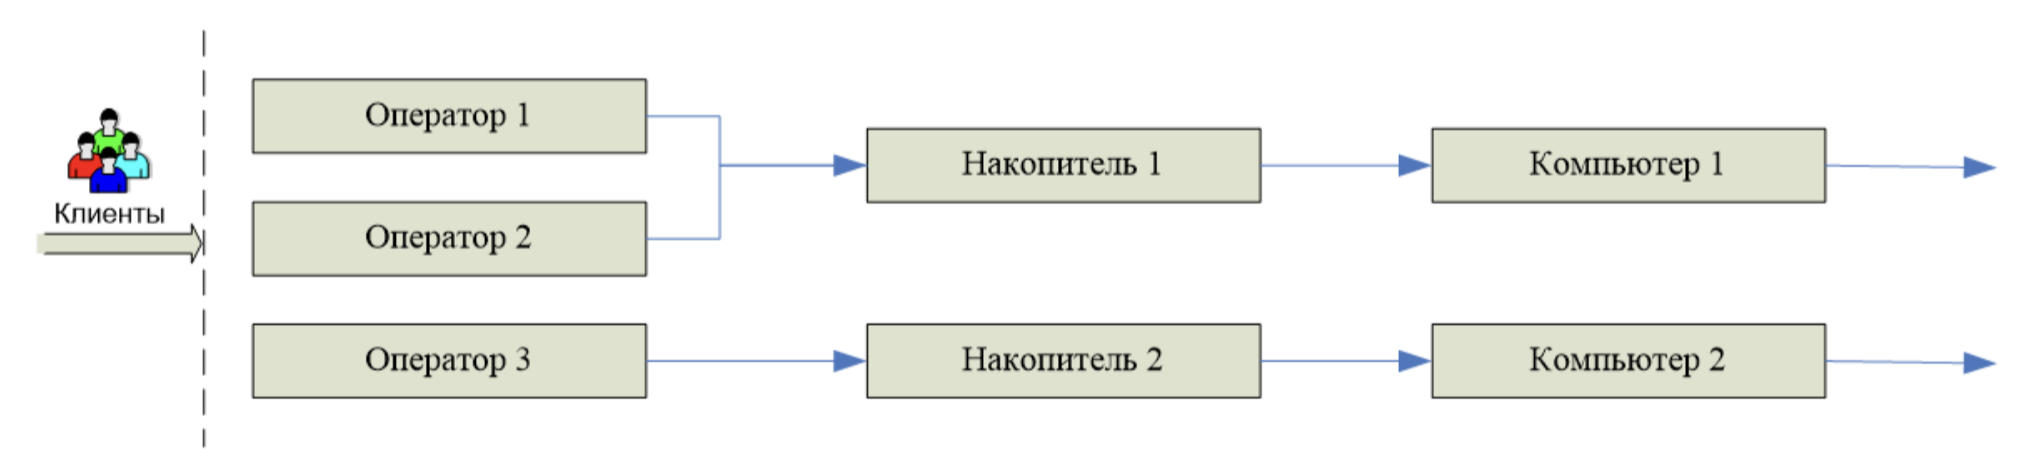
\includegraphics[scale=0.4]{schema}
\end{figure}

\section{{Теоритическая часть}}
\hspace*{5mm} В процессе взаимодействия клиентов с информационным центром возможно:
\begin{itemize}
	\item режим нормального обслуживания, т.е. клиент выбирает одного из свободных операторов, отдавая предпочтение тому у которого меньше номер;
	\item режим отказа в обслуживании клиента, когда все операторы заняты. 
\end{itemize}
\textbf{Переменные и уравнения имитационной модели }
\\ \hspace*{5mm} Эндогенные переменные: время обработки задания i-ым оператором, время решения этого задания j-ым компьютером.
\clearpage
\newpage
\hspace*{5mm}  Экзогенные переменные: число обслуженных клиентов и число клиентов, получивших отказ.
\begin{figure}[h!]
	\centering 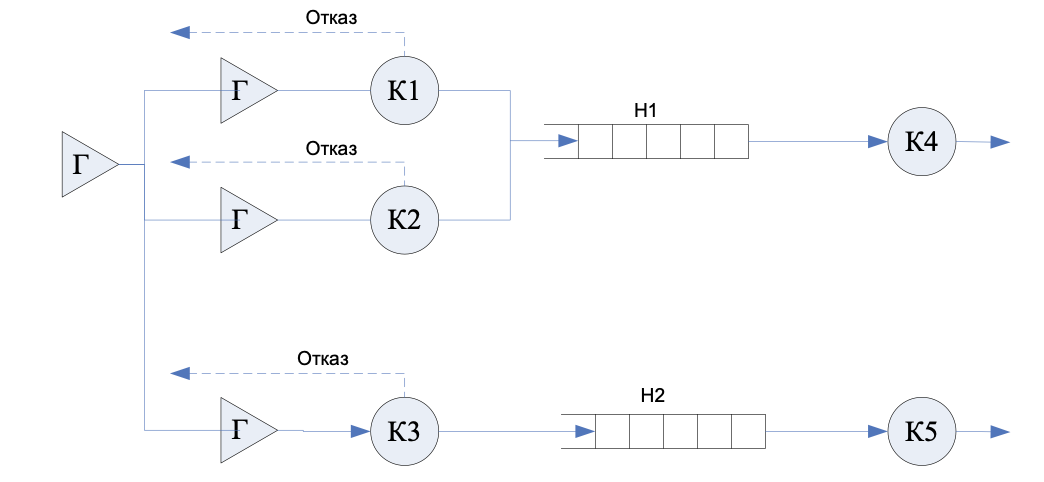
\includegraphics[scale=0.7]{schema1}
\end{figure}

\section{{Результаты}}
На рисунке ниже показаны результаты обработки 300 заявок информационным центорм при помощи языка GPSS. Можно заметить что из 300 заявок были отклонены только 23\%.
\begin{figure}[h!]
	\centering 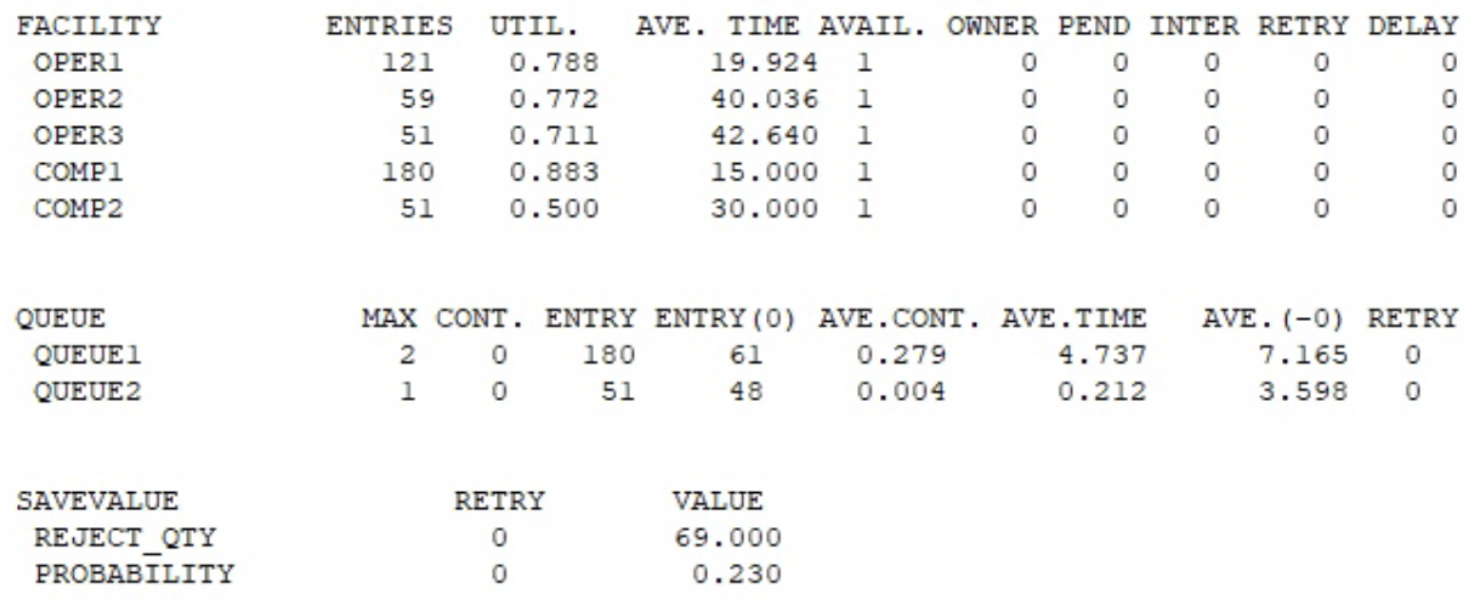
\includegraphics[scale=0.5]{gpss}
\end{figure}
\\ Ниже показаны результаты моделирования идентичного информационного центра, но на языке Python3.  Полученные результаты близки к результатам моделирования с помощью языка GPSS. 
\begin{figure}[h!]
	\centering 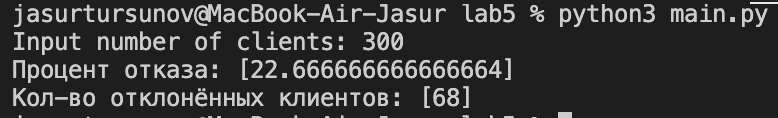
\includegraphics[scale=1]{300}
\end{figure}

\section{Листинг кода}
\begin{figure}[h!]
	\centering 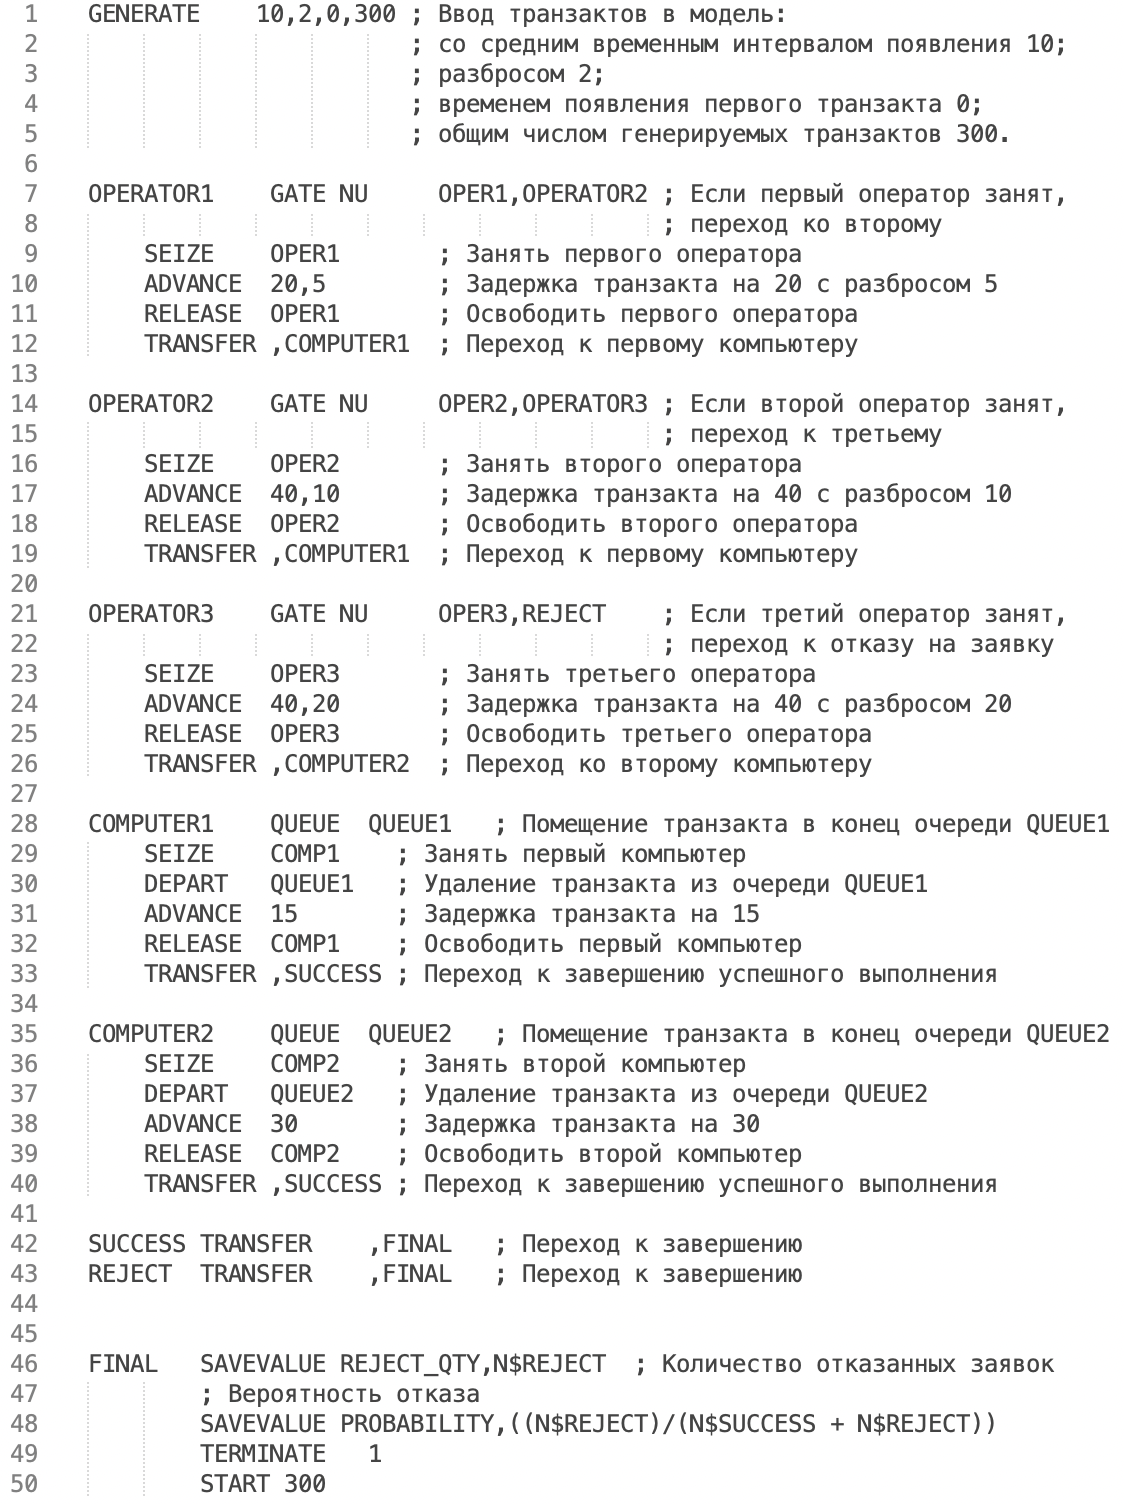
\includegraphics[scale=0.8]{listing}
\end{figure}
\end{document}